\documentclass[letterpaper,12pt]{article}
\usepackage{float}
\usepackage{array}
\usepackage{threeparttable}
\usepackage{geometry}
\geometry{letterpaper,tmargin=1in,bmargin=1in,lmargin=1.25in,rmargin=1.25in}
\usepackage{fancyhdr,lastpage}
\pagestyle{fancy}
\lhead{}
\chead{}
\rhead{}
\lfoot{}
\cfoot{}
\rfoot{\footnotesize\textsl{Page \thepage\ of \pageref{LastPage}}}
\renewcommand\headrulewidth{0pt}
\renewcommand\footrulewidth{0pt}
\usepackage[format=hang,font=normalsize,labelfont=bf]{caption}
\usepackage{listings}
\lstset{frame=single,
  language=Python,
  showstringspaces=false,
  columns=flexible,
  basicstyle={\small\ttfamily},
  numbers=none,
  breaklines=true,
  breakatwhitespace=true
  tabsize=3
}
\usepackage{amsmath}
\usepackage{amssymb}
\usepackage{amsthm}
\usepackage{harvard}
\usepackage{setspace}
\usepackage{float,color}
\usepackage[pdftex]{graphicx}
\usepackage{hyperref}
\hypersetup{colorlinks,linkcolor=red,urlcolor=blue}
\theoremstyle{definition}
\newtheorem{theorem}{Theorem}
\newtheorem{acknowledgement}[theorem]{Acknowledgement}
\newtheorem{algorithm}[theorem]{Algorithm}
\newtheorem{axiom}[theorem]{Axiom}
\newtheorem{case}[theorem]{Case}
\newtheorem{claim}[theorem]{Claim}
\newtheorem{conclusion}[theorem]{Conclusion}
\newtheorem{condition}[theorem]{Condition}
\newtheorem{conjecture}[theorem]{Conjecture}
\newtheorem{corollary}[theorem]{Corollary}
\newtheorem{criterion}[theorem]{Criterion}
\newtheorem{definition}[theorem]{Definition}
\newtheorem{derivation}{Derivation} % Number derivations on their own
\newtheorem{example}[theorem]{Example}
\newtheorem{exercise}[theorem]{Exercise}
\newtheorem{lemma}[theorem]{Lemma}
\newtheorem{notation}[theorem]{Notation}
\newtheorem{problem}[theorem]{Problem}
\newtheorem{proposition}{Proposition} % Number propositions on their own
\newtheorem{remark}[theorem]{Remark}
\newtheorem{solution}[theorem]{Solution}
\newtheorem{summary}[theorem]{Summary}
%\numberwithin{equation}{section}
\bibliographystyle{aer}
\newcommand\ve{\varepsilon}
\newcommand\boldline{\arrayrulewidth{1pt}\hline}


\begin{document}

\begin{flushleft}
  \textbf{\large{Problem Set \#3}} \\
  MACS 30000, Dr. Evans \\
  Alice Mee Seon Chung
\end{flushleft}

\vspace{5mm}

\noindent\textbf{Problem 1: A lifetime of temperatures}
 
 \textbf \\ Plot the scatter plot of maximum and minimum temperature for each day of Ricardo's life. 
 
\begin{figure}[H]\centering\captionsetup{width=5.0in}
  \caption{\textbf{Scatter Plot }}\label{Fig_1}
  \fbox{\resizebox{5.5in}{4.0in}{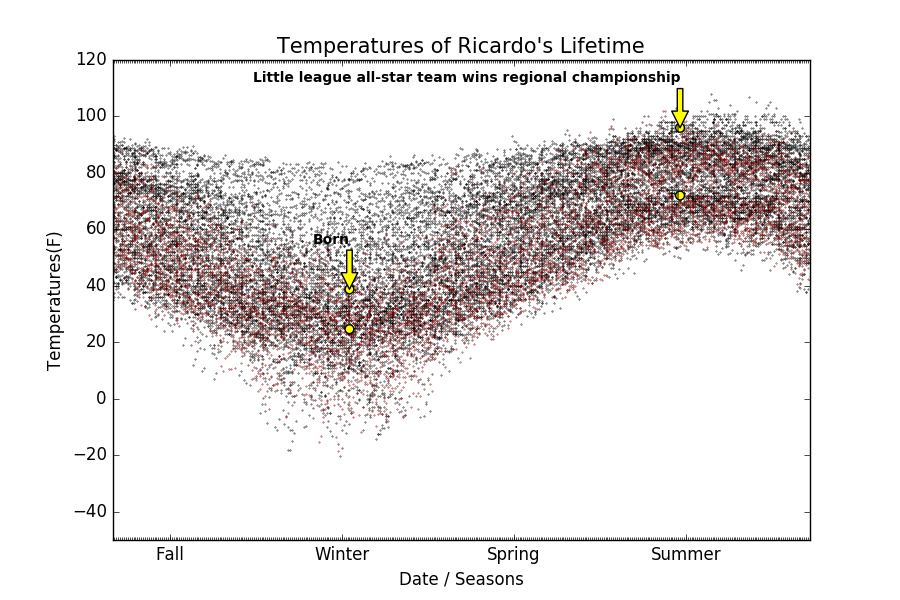
\includegraphics{Fig_1.png}}}
 \end{figure}
 \newpage
 
 
\noindent\textbf{Problem 2: 3D histogram}
 \textbf \\  
 \\ {(a)} Make a 2D  frequency histogram with 25 equally spaced bins. 
 \begin{figure} [H]\centering\captionsetup{width=4.0in}
  \caption{\textbf{The 2D histogram}}\label{Fig_2a}
  \fbox{\resizebox{5.0in}{4.0in}{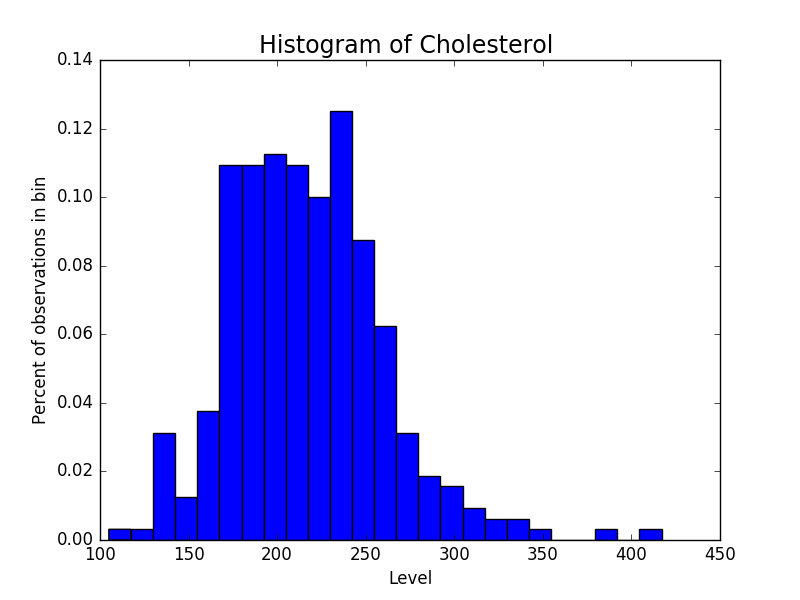
\includegraphics{Fig_2a.png}}}
 \end{figure}
 
 \textbf \\Question a.  What is the midpoint of the bin with the highest frequency? 
            \\
           \\ Answer: The midpoint of 2d histogram of Cholesterol is 236.04.

\newpage
 
 \textbf \\  
 \\ {(b)} Make a 3D frequency histogram with 25 equally spaced bins in both the cholesterol and trigliceride dimensions.
 \begin{figure} [H]\centering\captionsetup{width=4.0in}
  \caption{\textbf{The 3D histogram}}\label{Fig_2b}
  \fbox{\resizebox{5.0in}{4.0in}{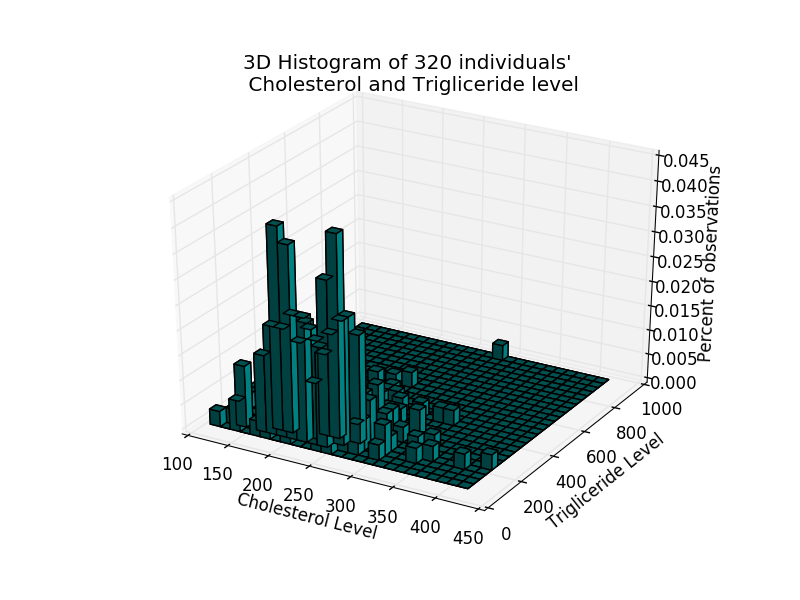
\includegraphics{Fig_2b.png}}}
 \end{figure}�

 \textbf \\Question b. What is the key new characteristic that emerges from the data?
             \\
              \\ Answer: The key new characteristics that emerges from the data is Trigliceride. 
             \\ Trigliceride has different highest bin compared to Cholesterol and it has lower level than Cholesterol. 
             Combined with two data set, many individuals who have evidence of heart disease seem to have relatively low Trigliceride level under 200 andCholesterol level from 150 to 250 level.
             \\
             \\Question c. If you had to interpret the findings from the 3D histogram, what group or groups might you say have the highest risk for heart disease?
             \\
             \\ Answer: As seen in the Fig 2b, the groups might have the highest risk of heart disease in the graph have relatively low level of Trigliceride like under 200 level and relatively low to mid level of Cholesterol like approximately from 150 to 250 level.
             
\newpage

\noindent\textbf{Problem 3: Comparing segments of time series}
\textbf \\  
 \\ Plot each of the 14 segments of the normalized job growth data series that start one year before the peak date of the recession and end seven years after
the recession as a line plot.
 \begin{figure} [H]\centering\captionsetup{width=4.0in}
  \caption{\textbf{Line Plot}}\label{Fig_3}
  \fbox{\resizebox{6.5in}{4.5in}{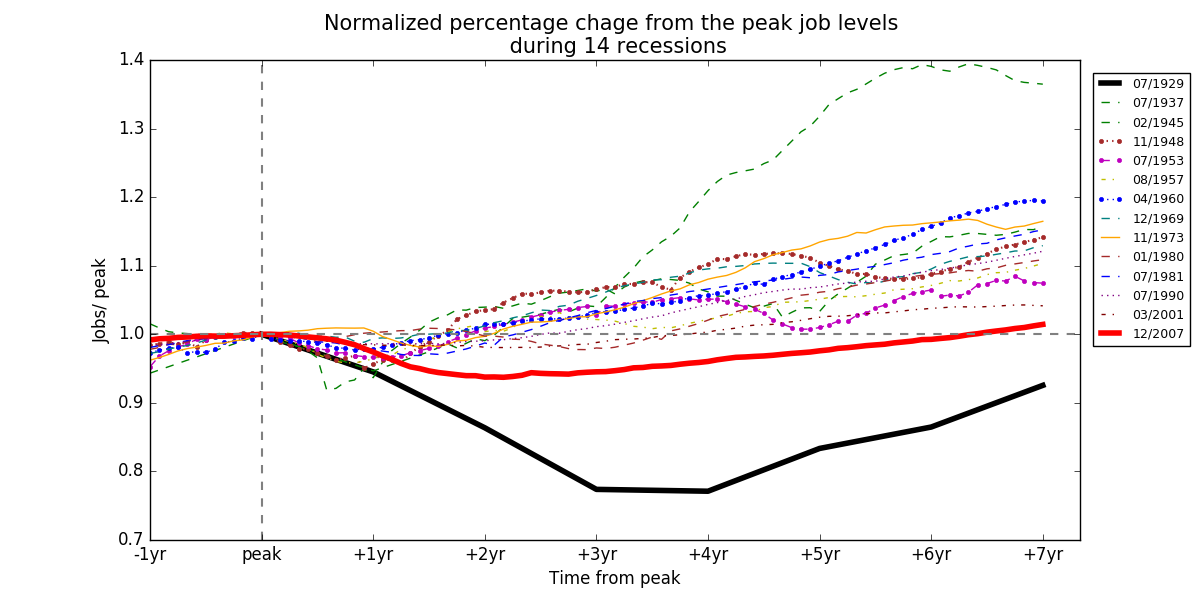
\includegraphics{Fig_3.png}}}
 \end{figure}�

 \textbf \\Question j. What is the key new characteristic that emerges from the data?
             \\
              \\ Answer: In the short term like the period from peak year to 1 year later,there are several U.S recessions worse than the Great Recession in terms of jobs beside the Great Depression, but in the long term through 9 years after, other recessions beside the Great Depression recovered above the peak year's job level faster than the Great Recession. So we can say there are any U.S recessions worse than the Great Recession in terms of jobs beside the Great Depression. 
 \newpage
 
 \textbf \\  
              \\ Question j. Are there any ways in which the Great Recession has been worse than the Great Depression in the United States?
              \\
              \\ Answer: As you seen in the Fig 3 graph, there are any ways in which the Great Recession has been worse than the Great Depression in the U.S. The Great Depression job level kept fall down for almost 3 years and started to recover slowly and even 9 years after the job level could not recover to the peak year job level.  

              


\end{document}
